% !TEX TS-program = pdflatex
% !TeX program = pdflatex
% !TEX encoding = UTF-8
% !TEX spellcheck = fr

\documentclass[11pt, a4paper]{article}
%\usepackage{fullpage}
\usepackage[left=1cm,right=1cm,top=1cm,bottom=2cm]{geometry}
\usepackage[fleqn]{amsmath}
\usepackage{amssymb}
%\usepackage{indentfirst}
\usepackage[T1]{fontenc}
\usepackage[utf8]{inputenc}
\usepackage[french,english]{babel}
\usepackage{txfonts} 
\usepackage[]{graphicx}
\usepackage{multirow}
\usepackage{hyperref}
\usepackage{parskip}
\usepackage{multicol}
\usepackage{wrapfig}

\usepackage{turnstile}%Induction symbole

\usepackage{tikz}
\usetikzlibrary{arrows, automata}
\usetikzlibrary{decorations.pathmorphing}

\renewcommand{\baselinestretch}{1}

\setlength{\parindent}{24pt}


\begin{document}

\selectlanguage {french}
%\pagestyle{empty} 

\noindent
\begin{tabular}{ll}
\multirow{3}{*}{
\includegraphics[width=2cm]{../img/esi-logo.png}} & \'Ecole national Supérieure d'Informatique\\
& 2\textsuperscript{ème} année cycle supérieure (2CSSIL2, 2CSSIQ2)\\
& Machine Learning (2022-2023)
\end{tabular}\\[.25cm]
\noindent\rule{\textwidth}{1pt}\\%[-0.25cm]
\begin{center}
{\LARGE \textbf{Workshop: Réseaux de neurones avances}}
\begin{flushright}
	ARIES Abdelkrime
\end{flushright}
\end{center}
\noindent\rule{\textwidth}{1pt}

\section*{Information}

\begin{itemize}
	\item Dataset : Pokemon Image Dataset : {\scriptsize\url{https://www.kaggle.com/datasets/vishalsubbiah/pokemon-images-and-types}}
	\item Il n'y a pas des spécifications pour construire les architectures : l'étudiant est libre à utiliser les composants vus dans le tutoriel : {\scriptsize \url{https://github.com/projeduc/ESI_2CS_ML/tree/main/tuto/NN}}
	\item Le pré-traitement est fourni avec ce lab (il faut renommer le dossier comme "pokemon" ou changer le chemin du dataset dans le code fourni)
\end{itemize}

\section{Classement CNN}

\begin{itemize}
	\item Concevoir un modèle qui classe les pokémons selon leurs type selon les spécifications de la figure \ref{fig:CNN-pok-cls}.
	\item Entraîner le modèle avec validation en calculant l'accuracy.
	\item Dessiner l'évolution des coûts (entrainement et validation).
	\item Calculer la précision et rappel sur le dataset de test.
	\item Essayer de proposer une autre architecture pour améliorer la performance en terme de précision et rappel.
\end{itemize}

\begin{figure}[htp]
	\centering
	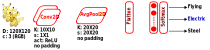
\includegraphics[width=0.8\textwidth]{../img/workshop/CNN-pok-cls.pdf}
	\caption{Architecture de classement Pokemon basée sur les CNN}
	\label{fig:CNN-pok-cls}
\end{figure}

\section{Auto-encodeur de clustering}

\begin{itemize}
	\item Concevoir le modèle illustré dans la figure \ref{fig:MLP-pok-cluster}. 
	Ici, nous voulons représenter chaque Pokemon par un vecteur de deux éléments.
	\item Générer les codes des Pokemons d'entrainement.
	\item Ploter leurs positions en se basant sur ce code en indiquant leurs types.
	\item Appliquer K-Means sur les Pokemons d'entrainement en se basant sur leurs codes. 
	Ici, K est le nombre des classes.
	\item Pour chaque cluster généré, nous supposons que la classe majoritaire est celle représentée par ce cluster.
	\item Calculer l'indice de Rand : \textbf{sklearn.metrics.rand\_score}
	\item Répéter la même chose avec un auto-encodeur CNN.
\end{itemize}

\begin{figure}[htp]
	\centering
	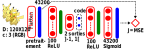
\includegraphics[width=0.6\textwidth]{../img/workshop/MLP-pok-cluster.pdf}
	\caption{Architecture de regroupement des Pokemons en utilisant un MLP.}
	\label{fig:MLP-pok-cluster}
\end{figure}


\section{Auto-encodeur de clustering pour classement}

Concevoir un modèle qui prend le code généré par l'auto-encodeur précédent et classe le pokémon selon son type : 
\begin{itemize}
	\item Il faut utiliser l'encodeur entraîné précédemment ; c-à-d. L'entrée doit être une image et pas le vecteur de son code.
	\item Le modèle est un MLP (obviously!) qui prend la sortie de l'encodeur comme entrée et qui génère le type du pokémon.
	\item Lors de l'entraînement du classeur, il ne faut pas mettre à jours l'encodeur ; il faut désactiver l'entraînement du modèle : \textbf{model.trainable = False}.
	\item Comparer entre ce modèle et celui du classement CNN.
\end{itemize}

\section*{Génération des images}

Concevoir un modèle qui génère des nouveaux pokémons en suivant les spécifications suivantes : 
\begin{itemize}
	\item Le code est un vecteur de 10 à 50 éléments (au choix).
	\item Deux architectures: Auto-encodeur variationnelle et GAN.
	\item De préférence, utiliser des CNN.
	\item De préférence, utiliser la classe du pokémon afin d'apprendre la génération. C-à-d, l'entrée du décodeur doit être un code aléatoire fusionné avec le code one-hot de la classe.
\end{itemize}


\end{document}
